\chapter{Travaux réalisés}
Cette partie présente les travaux réalisé dans ce projet.  Puisqu'il y a une grosse partie de travail qui concerne les nombreux tests et les analyses donc un autre chapitre indépendent est créé pour la présenter.

\section{Finition de la méthode heuristique de liste (H1)}%%%%%%%%%%%%%%%%%%%%%%%%
Les algorithmes et le programme de H1 ont été principalement réalisés par Cyrille PICARD avant ce projet. Cependant, ce travail n'a pas été vraiment fini et il existe des problèmes dans les algorithmes ainsi que dans l'implémentation.

Les travaux réalisés concernent donc la correction des algorithmes ainsi que ses implémentations. Cette partie a duré plus longtemps que ce que nous avions prévu. Finalement la partie principale du programme est quasiment réécrit. La plus part de travail se porte sur la programmation C++ qui n'est pas très pertinent d'être présentée dans ce rapport. Par contre, nous listons ici les algorithmes (pseudo-code) principals que nous avons créés ou modifiés.

\subsection{Algorithmes}%%%%%%%%%%%%%%%%%%%%%%%%%%
Nous listons dans cette section les algorithmes critiques de la méthode H1. Nous avons fait des efforts pour rendre la présentation assez synthétique et compréhensible.

Avant d'entrer dans les algorithmes, nous déclarons ici des structrues de données globales qui peuvent être utilisées sans déclaration dans n'importe quel algorithme.

\begin{enumerate}
	\item ListeGPU1: la liste des tâches non-préemptable ayant des besoins en GPU et CPU et tel que besoins HDD > besoins RAM.
	\item ListeGPU2: la liste des tâches non-préemptable ayant des besoins en GPU et CPU et tel que besoins HDD < besoins RAM.
	\item ListeCPU1: la liste des tâches non-préemptable ayant des besoins uniquement en CPU et tel que besoins HDD > besoins RAM.
	\item ListeCPU2: la liste des tâches non-préemptable ayant des besoins uniquement en CPU et tel que besoins HDD < besoins RAM.
	\item ListeTachesPr: la liste de toutes les tâches préemptable.
	\item ListePrGPU1: la liste des tâches préemptable ayant des besoins en GPU et CPU et tel que besoins HDD > besoins RAM.
	\item ListePrGPU2: la liste des tâches préemptable ayant des besoins en GPU et CPU et tel que besoins HDD < besoins RAM.
	\item ListePrCPU1: la liste des tâches préemptable ayant des besoins uniquement en CPU et tel que besoins HDD > besoins RAM.
	\item ListePrCPU2: la liste des tâches préemptable ayant des besoins uniquement en CPU et tel que besoins HDD < besoins RAM.
	\item ListeOrdo: la liste de l'ordonnancement en sortie.
\end{enumerate}
\bigskip

Le premier algorithme\ref{algo0} est l'algorithme général qui est le plus synthétique. L'idée de l'algorithme\ref{algo1} est de déterminer les intervalles \textit{stable}, c'est-à-dire toutes les tâches du même intervalle ontle même Ui (prévue à être exécutée).
L'algorithme CréerListeServeurTriée\ref{algo2} trie la liste des serveurs selon le coût normalisé croissant.
L'algorithme TrierTâches\ref{algo4} trie la liste de tâches selon leur priorités pour un intervalle et une machines donnée.
L'algorithme Ordonnancer\ref{algo5} effectue l'ordonnancement. L'algorithme AllumageMachine\ref{algo7} détermine est-ce qu'on peut rallumer une machine pour mettre la tâche, si oui c'est la quelle.

\begin{algorithm}[H]
\caption{Algorithme Général}
\label{algo0}
\algsetup{indent=3em}
\begin{algorithmic}[1]
\REQUIRE {
\STATE ListOrdo: le tableau qui contient la matrice d'affectation des VMs sur les machines phisiques.
\STATE IsFeasible: booléan qui indique si on a bien ordonnancé toutes les tâches non-préemptables.
\STATE coûtTotal: le coûtTotal selon l'ordonnancement effectué.
}
\ENSURE {
\STATE ListOrdo, IsFeasible, coûtTotal
}
\LOOP
\STATE IsFeasible = true;
\STATE CalculerIntervalle();
\STATE CréerListeServeurTriée();
	\FOR{chaque intervalle i}
		\STATE CréerListesTâche(i);
		\STATE Ordonnancer(ListeOrdo, i);
	\ENDFOR
\STATE	
\COMMENT {Maintenant on a fini l'ordonnancement des tâches et on peut déjà calculer le coût total.}
\STATE coûtTotal = CalculerCoûtTotal();
\STATE
\COMMENT {Voir si la solution est feasable}
	\FOR{ chaque intervalle i }
		\FOR{ chaque tâche t }
			\IF{(t n'est pas préemptable ET ListeOrdo[i][t] == -1) }
			\STATE IsFeasible = false;
			\RETURN;
			\ENDIF
		\ENDFOR
	\ENDFOR
\ENDLOOP
\end{algorithmic}
\end{algorithm} 

%%%%%%%%%%%%%%%%%%%%%% Algo 1 %%%%%%%%%%%%%%%%%%%

\begin{algorithm}[H]
\caption{CaculerIntervalle}
\label{algo1}
\algsetup{indent=3em}
\begin{algorithmic}[1]
\ENSURE {
\STATE	ListeIntervalle: le tableau des intervalles trouvés
}\\
%\BEGIN
\LOOP
\STATE Entier nbIntervalle=0;
\STATE ListeIntervalle[0].BorneInf = 0;
\STATE ListeIntervalle[0].BorneSup = 0;
	\FOR{ t allant de 0 à T-2 }
		\FOR{ iTache allant de 0 à N-1 }
			%\COMMENT{Intervalle trouvé}
			\IF{ u(iTache,t)!=u(iTache,t+1) }  
				\STATE nbIntervalle = nbIntervalle+1;
				\STATE ListeIntervalle[nbIntervalle-1].BorneSup = t;
				%\COMMENT{Intervalle suivant}
				\STATE ListeIntervalle[nbIntervalle].BorneInf = t+1; 
				\STATE break;
			\ENDIF
		\ENDFOR
	\ENDFOR
	\STATE nbIntervalle=nbIntervalle+1;
	\STATE ListeIntervalle[nbIntervalle-1].BorneSup = T-1;
\ENDLOOP
%\END
\end{algorithmic}
\end{algorithm} 

%%%%%%%%%%%%%%%%%%%%%% Algo 2 %%%%%%%%%%%%%%%%%%%

\begin{algorithm}[H]
\caption{CréerListeServeurTriée}
\label{algo2}
\algsetup{indent=3em}
\begin{algorithmic}[1]
\ENSURE {
\STATE	ListeServeur: le tableau des serveurs triés par ordre croissant en fonction du coût normalisé
}\\
\LOOP
	\STATE Réel CoutTotal, SommeCaract;
	\FOR {i allant de 0 à M-1 }
		\STATE ListeServeur[i].IndiceServeur=i;
		\STATE CoutTotal=mc(i)*alphac(i) +mg(i)*alphag(i) + mr(i)*alphar(i)+ mh(i)*alphah(i);
		\STATE SommeCaract = mc(i)+mg(i)+mr(i)+mh(i);
		\STATE ListeServeur[i].CoutNorm = CoutTotal / SommeCaract ;
	\ENDFOR
	\STATE TrierParCoutNorm(ListeServeur);
\ENDLOOP
\end{algorithmic}
\end{algorithm}


%%%%%%%%%%%%%%%%%%%%%%%%%% Algo 3 (567) %%%%%%%%%%%%%%%%%%%%%%

\begin{algorithm}[H]
\caption{CréerListesTâches}
\label{algo3}
\algsetup{indent=3em}
\begin{algorithmic}[1]
\REQUIRE {
	\STATE indice: l'indice de l'intervalle sur lequel on travaille
}
\ENSURE {
	\STATE ListeTachesPr: la liste des tâches préemptable.
	\STATE \COMMENT{Les tâches sont réparties dans ces 8 listes selon leurs besoins en GPU, CPU, HDD, RAM et si la tâche est préemptable.}
	\STATE ListeGPU1, ListeCPU1, ListePrGPU1, ListePrCPU1 //Tâches non-préenptables
	\STATE ListeGPU2, ListeCPU2, ListePrGPU2, ListePrCPU2 //Tâches préenptables
}
\LOOP
	\FOR{ tâche de 0 à N()-1 }
		\IF{(u(tâche, temps)=1) } 
			\STATE \COMMENT{Cette tâche peut être exécutée en ce moment}
			\IF{ (R(tâche==0))	}
				\IF{(ng(tâche)>0) }
					\IF{(nh(tâche) > nr(tâche)) }
						\STATE Répartir cette tâche à ListeGPU1;
					\ELSE
						\STATE Répartir cette tâche à ListeGPU2;
					\ENDIF
				\ELSE	
					\STATE \COMMENT{ng(tâche)=0}
					\IF{(nh(tâche) > nr(tâche)) }
						\STATE Répartir cette tâche à ListeCPU1;
					\ELSE
						\STATE Répartir cette tâche à ListeCPU2;
					\ENDIF
				\ENDIF
			\ELSE	
				\STATE \COMMENT{Cette tâche est préemptable}
				\STATE Répartir cette tâche à ListeTâchesPr;
				\IF{(ng(tâche)>0) }
					\IF{(nh(tâche) > nr(tâche)) }
						\STATE Répartir cette tâche à ListePrGPU1;
					\ELSE
						\STATE Répartir cette tâche à ListePrGPU2;
					\ENDIF
				\ELSE	
					\STATE \COMMENT{ng(tâche)=0}
					\IF{(nh(tâche) > nr(tâche)) }
						\STATE Répartir cette tâche à ListePrCPU1;
					\ELSE
						\STATE Répartir cette tâche à ListePrCPU2;
					\ENDIF
				\ENDIF
			\ENDIF
		\ENDIF
	\ENDFOR
\ENDLOOP
\end{algorithmic}
\end{algorithm} 



%%%%%%%%%%%%%%%%%%%%%%%%%% Algo 4 (8) %%%%%%%%%%%%%%%%%%%%%%

\begin{algorithm}[H]
\caption{TrierTâches}
\label{algo4}
\algsetup{indent=3em}
\begin{algorithmic}[1]
\REQUIRE {
	\STATE indice: indice de l'intervalle
	\STATE indiceServeur: indice de la machine
	\STATE list: une liste de tâches à trier
	\STATE taille: la taille de la liste
}
\ENSURE {
	\STATE list: liste de tâches triée par prio décroissant
}
\LOOP
	\STATE Entier IB;
	\STATE Entier WG;
	\STATE Entier MachineRecevoir;
	\COMMENT{La durée d'exécution actuelle de la tâche}
	\STATE Entier duree;	
	
	\FOR{ iboucle de 0 à taille }
		\STATE list[iboucle].prio = 0;
		\STATE IB = 0;
		\STATE WG = 0;
		\STATE MachineRecevoir = 0;

		\STATE duree = GetDureeExeActuelle(indice, list[iboucle].IndiceVM);
		\IF{ (la tâche n'est pas encore affectée) }
			\IF{ (cette tâche était affectée sur cette machine à l'intervalle précédent) }
				\STATE \COMMENT{La tâche a plus de priorité }
				\STATE IB = M();	
			\ENDIF
			\STATE \COMMENT{Si migration pas possible}
			\IF{ (duree!=0 et duree<mt(list[iboucle].IndiceVM)) }		
				\STATE Chercher indiceInterval qui est le dernier intervalle où la tâche était exécutée.
				\IF{ (indiceInterval est trouvé et la machine correspondante est la même) }
					\STATE WG = indiceServeur;
				\ELSE
					\STATE \COMMENT{ça veut dire pas possible}
					\STATE WG = -M(); 	
				\ENDIF
			\ELSE
				\FOR{ iboucle2 de 0 à <M() }
					\IF{ (ListeMachine[iboucle2] peut recevoir la tâche) }
						\STATE MachineRecevoir++;
					\ENDIF
				\ENDFOR
					\STATE WG = M() -  MachineRecevoir;
			\ENDIF
			\STATE list[iboucle].prio = IB + WG;
		\ENDIF
		\STATE \COMMENT{Trier les tâches en priorité décroissante}
		\STATE SortListByPrio(list);
	\ENDFOR
\ENDLOOP
\end{algorithmic}
\end{algorithm} 


%%%%%%%%%%%%%%%%%%%%%%%%%% Algo 5 %%%%%%%%%%%%%%%%%%%%%%
\begin{algorithm}[H]
\caption{Ordonnancer}
\label{algo5}
\algsetup{indent=3em}
\begin{algorithmic}[1]
\REQUIRE {
	\STATE indiceInter: L'intervalle à traiter.
}
\ENSURE {
	\STATE ListeOrdo: Une variable globale qui représente le résultat de l'ordonnancement.
}
\LOOP
		\STATE indiceAllume: L'indice de la machine qui sera allumée
	\STATE \COMMENT{Affecter d'abord les tâches non préemptables}
	\FOR{ indiceServeur de 0 à NbServeur }
		\IF{ (toute les tâches non-préemptables sont affectées) }
			\STATE break;
		\ENDIF
		
		\STATE \COMMENT{Ordonnancer les tâches non-préemptables sur le serveur indiceServeur}
		\STATE TrierTâches(ListeGPU1, indiceServeur);
		\STATE TrierTâches(ListeGPU2, indiceServeur);
		\STATE TrierTâches(ListeCPU1, indiceServeur);
		\STATE TrierTâches(ListeCPU2, indiceServeur);
		\STATE OrdoListeTache(ListeGPU1, indiceInter, indiceServeur, true);
		\STATE OrdoListeTache(ListeGPU2, indiceInter, indiceServeur, true);
		\STATE OrdoListeTache(ListeCPU1, indiceInter, indiceServeur, true);
		\STATE OrdoListeTache(ListeCPU2, indiceInter, indiceServeur, true);
		\STATE
		\STATE \COMMENT{Ordonnancer les tâches préemptables sur le serveur indiceServeur}
		\STATE TrierTâches(ListePrGPU1);
		\STATE TrierTâches(ListePrGPU2);
		\STATE TrierTâches(ListePrCPU1);
		\STATE TrierTâches(ListePrCPU2);
		\STATE OrdoListeTache(ListePrGPU1, indiceInter, indiceServeur, false);
		\STATE OrdoListeTache(ListePrGPU2, indiceInter, indiceServeur, false);
		\STATE OrdoListeTache(ListePrCPU1, indiceInter, indiceServeur, false);
		\STATE OrdoListeTache(ListePrCPU2, indiceInter, indiceServeur, false);
	\ENDFOR
	
	\STATE
	\STATE \COMMENT{Pour le reste des tâches prémptable, on regarde si on a besoin de rallumer des machines}
	\WHILE{ (Il y a encore des tâches préemptables non affectées) }
		\STATE indiceAllume = AllumageMachine(indiceInter);
		\IF{ (indiceAllume==-1) }
			\STATE \COMMENT{Aucune machine ne peut être allumée, arrêter.}
			\RETURN;
		\ELSE
			\STATE TrierTâches(ListePrGPU1);
			\STATE TrierTâches(ListePrGPU2);
			\STATE TrierTâches(ListePrCPU1);
			\STATE TrierTâches(ListePrCPU2);
			\STATE OrdoListeTache(ListePrGPU1, indiceInter, indiceServeur, true);
			\STATE OrdoListeTache(ListePrGPU2, indiceInter, indiceServeur, true);
			\STATE OrdoListeTache(ListePrCPU1, indiceInter, indiceServeur, true);
			\STATE OrdoListeTache(ListePrCPU2, indiceInter, indiceServeur, true);
		\ENDIF
	\ENDWHILE
\ENDLOOP
\end{algorithmic}
\end{algorithm}



%%%%%%%%%%%%%%%%%%%%%%%%%% Algo 6 %%%%%%%%%%%%%%%%%%%%%%
\begin{algorithm}[H]
\caption{OrdoListeTache}
\label{algo6}
\algsetup{indent=3em}
\begin{algorithmic}[1]
\REQUIRE {
	\STATE ListeTâche: La liste des tâches.
	\STATE indiceI: L'indice d'intervalle.
	\STATE indiceS: L'indice du serveur.
	\STATE canTurnOn: un booléan pour indique quand le serveur n'est pas allumé est-ce qu'on a le droit de l'allumer et affecter au-dessus.
}   
\ENSURE {
	\STATE ListeOrdo: L'affectation des tâches est enregistrée dans cette liste qui est aussi la sortie du programme.
}
\LOOP
	\STATE Entier interInf, interSup, indiceVM, indiceVM2;
	\STATE Entier dureeExeActuelle;
	\STATE interInf = ListeIntervalle[indiceI].BorneInf;
	\STATE interSup = ListeIntervalle[indiceI].BorneSup;
	\STATE 
	\FOR{ chaque tâche t dans ListTâche }
		\IF{(t n'est pas encore affectée sur cet intervalle) }
			\IF{(Le serveur indiceS possède assez de ressource pour t) }
				\FOR{ chaque tâche t2 qui a une affinité avec t et qui a été affectée sur un autre serveur indiceS2 }
					\IF{( false == CalculFesabiliteReseau(t1.indiceVM, t2.indiceVM, indiceS, indiceS2, indiceI) ) }
						\STATE Cette tâche t ne peut pas affectée sur ce serveur, car le réseau ne le permet pas.
						\STATE Continuer voir la tâche suivante dans ListTâche.
					\ENDIF
				\ENDFOR
				\STATE 
				\STATE \COMMENT{Maintenant on est sûr que la tâche peut être affectée, alors on l'affecte...}
				\STATE MaJReseau(t1.indiceVM, t2.indiceVM, indiceS, indiceS2, indiceI);
				\FOR{ chaque instant de temps i }
					\STATE Mettre à jour ListeOrdo[i][t.indiceVM];
					\STATE Mettre à jour les caractéristiques de ce serveur(indiceS);
				\ENDFOR
			\ENDIF
		\ENDIF
	\ENDFOR
\ENDLOOP
\end{algorithmic}
\end{algorithm} 


%%%%%%%%%%%%%%%%%%%%%%%%%% Algo 7 %%%%%%%%%%%%%%%%%%%%%%
\begin{algorithm}[H]
\caption{AllumageMachine}
\label{algo7}
\algsetup{indent=3em}
\begin{algorithmic}[1]
\REQUIRE {
	\STATE indiceInter: L'intervalle à traiter.
}   
\ENSURE {
	\STATE indiceAllume: indice de la machine à allumer. -1 s'il y en a pas.
}
\LOOP
	\STATE inf: instant inférieur de l'intervalle
	\STATE sup: instant supérieur de l'intervalle
	\STATE critère: la différence entre le coût de rallumer la machine et le coût de ne pas la rallumer. Plus c'est moins, mieux c'est.
	\STATE critèreMin: le minimum du critère.
	\STATE
	\STATE inf = ListeIntervalles[indiceInter].BorneInf;
	\STATE sup = ListeIntervalles[indiceInter].BorneSup;
	\STATE critèreMin = 0;
	\FOR{  chaque machine m }
		\IF{ (m n'est pas allumée) }
			\STATE critère = (sup - inf + 1) * beta(m); //Le coût d'être ON
			\FOR{  (chaque tâche t préemptable qui n'est pas encore affectée) }
				\IF{ (m peut recevoir t) }
					\STATE critère = critère + (sup - inf + 1 ) * CalculCoutAffectation(t,m) - rho(t);
				\ENDIF
			\ENDFOR
			\IF{ (critère < critèreMin) }
				\STATE critèreMin  = critère;
				\STATE indiceAllume = m.indiceServeur;
			\ENDIF
		\ENDIF
	\ENDFOR
	
	\IF{(critèreMin < 0) }
		\RETURN indiceAllume;
	\ELSE
		\RETURN -1;
	\ENDIF
\ENDLOOP
\end{algorithmic}
\end{algorithm} 


\section{Réalisation de la méthode heuristique basée sur Cplex (H2)}%%%%%%%%%%%%%%%
La deuxième méthode heuristique est basée sur la méthode exacte du solveur Cplex. Il s'agit de chercher de bonnes valeurs de certains paramètres pour rendre la méthode en heuristique, qui peut nous donner une solution faisable (donc pas forcément optimale) dans un temps limité.

Les deux paramètres Cplex qui nous intéressent sont:
\begin{itemize}
	\item TimeLimit: durée maximum de résolution. Cplex s'arrête au bout de ce temps même s'il n'a pas encore trouver la solution optimale.
	\item EpGap: tolérance d’écart entre la solution trouvée et la borne inférieure. Si Cplex trouve une solution faisable qui n'est pas optimal mais qui est tolérée par cet écart alors il va aussi s'arrêter en retourner cette solution convenable.
\end{itemize}


\subsection{Détermination des paramètres}
Pour trouver de bonnes valeurs pour ces deux paramètres, nous avons réalisé une analyse sur les fichiers log Cplex engendrés pendant la résolution de certaines instances. En fait quand Cplex résoud un problème, il enregistre fréquemment les informations sur la déviation entre la solution actuelle et la LB, avec aussi le temps écoulé. A partir de ces informations, nous pouvons chercher la corrélation entre ces deux facteurs. La figure \ref{epgap} a été ensuite réalisée pour illustrer cette relation.

\begin{figure}[!htbp]
	\centering
		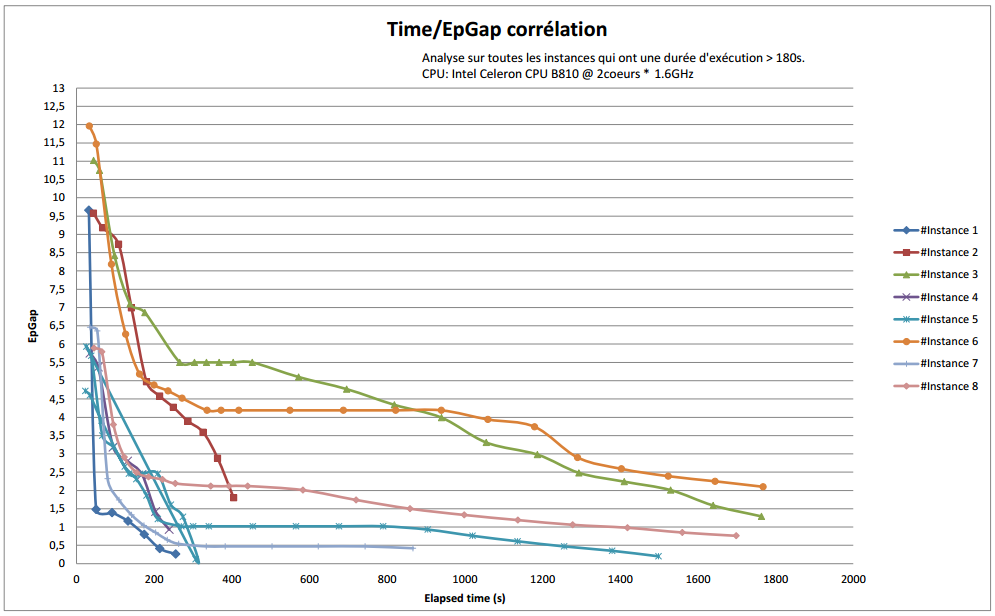
\includegraphics[scale=0.5]{pics/epgap.png}
	\caption{L'évolution de la déviation selon le temps écoulé}
	\label{fig:epgap}
\end{figure}
\bigskip
En analysant cette figure, nous avons choisi heuristiquement 2\% comme la valeur pour le paramètre \textit{EpGap} et 400s pour \textit{TimeLimit}. D'abord une déviation de 2\% reste très faible donc admissible, ensuite nous pouvons constater aussi après 400s la solution ne peut plus être améliorée facilement.

\section{Mise en oeuvre du Preprocessing}%%%%%%%%%%%%%%%%%%%%%%%%%%%%%%%%%%%%%
\subsection{Principe}
Le \textit{Preprocessing} est un prétraitement réalisé sur le modèle mathématique du problème avant de passer ce modèle au solveur. L'idée du Preprocessing est de fixer autant que possible de variables dans le modèle pour réduire la taille du problème et donc accélérer la résolution qui suit.

Pour le faire, il faut avoir une borne supérieure (UB) en entrée. Ça peut être fournit par les deux méthodes heuristiques que nous avons parlées. Ensuite il faut faire une relaxation continue sur le modèle pour obtenir un modèle LP dont les variables sont de type réel entre 0 et 1. 

Nous pouvons alors lancer la résolution LP sur ce modèle. La valeur objective obtenue est donc une borne inférieure (LB) du problème initial. Si toutes les variables de la solution valent 0 ou 1, alors le travail est fini ; sinon nous commenceons à fixer les variables qui ne sont pas entier de façons suivante: 

\begin{enumerate}
	\item Si le fait de fixer une variable à 0 va nous amener une solution qui viole la UB, alors il faut fixer cette variable à 1.
	\item Équalement, si le fait de fixer une variable à 1 va nous amener une solution qui viole la UB, alors il faut fixer cette variable à 0.
	\item S'il n'y a aucune variable qui peut être fixée, alors le Preprocessing est fini. Sinon il faut relancer la résolution LP et répéter le Preprocessing.
\end{enumerate}

Pour expliquer comment peut-on savoir un fixage à 0 ou à 1 peut violer la UB, il faut d'abord introduire les notions \textit{Reduced-cost} et \textit{Pseudo-cost}.

En effet après la résolution LP d'un problème, Cplex va attacher un \textit{Reduced-cost} à chaque variable qui est hors la \textit{Base}. Le \textit{Reduced-cost} signifie tout simplement l'influence d'un ajustement de la variable sur la valeur de la fonction objectif. Par exemple si nous voulons fixer à 1 une variable qui vaut 0.8, alors nous savons que la nouvelle valeur objective sera $sol+(1-0.8)*\textit{Reduced-cost}$ dont $sol$ est la valeur objective avant le fixage.

Le \textit{Pseudo-cost} a un sens similaire, mais c'est pour les variables qui sont dans la \textit{Base}.

Nous avons dejà une librairie C++ \textit{PreLib} qui est une implémentation de la technique du Preprocessing issue d'un autre projet. Pour l'employer dans ce projet, nous avons besoin de faire des adaptations, sinon la parite essentielle du Preprocessing est déjà prête à utiliser.

\subsection{Valide inequalities}
Selon l'analyse du premier test \ref{test_prep_nocut} du Preprocessing, nous avons constaté que les LBs pendant le Preprocessing ne sont pas assez proches de la solution optimale, ce qui gêne la performence du Preprocessing. Pour améliorer cette situation, nous décitons d'ajouter des \textit{Valide Inequalities} dans le modèle LP du problème.

Les \textit{Valide Inequalities} (ou Cut, Coupe) sont des contraintes supplémentaires qui sont redondantes, mais qui peuvent peut-être accélérer la résolution. Si ces coupes sont bien conçues, le solveur peut alors en profiter dans la procédure \textit{Branch \& Cut} pour éliminer très vite les branches inintéressantes ; mais l'ajout de ces coupes peut aussi amener un modèle grossi, ce qui peut au contraire ralentir la résolution. Donc le choix sur les coupes doit se faire avec modération. La conception, l'implémentation et le choix des coupes font une grande partie dans le travail de ce projet.

Nous distinguons deux types de coupe: la coupe dépendante du problème et la coupe classique qui ne dépend pas le problème. La premère coupe dépend la particularité du problème, elle est souvent sur l'utilisation des ressources. La coupe classique est inventée à partir des contraites existantes d'une façons mathématique. Dans les deux sections qui suivent, nous présentons une coupe dépendante du problème et une coupe classique que nous avons créé.

\subsubsection{Cuts sur les contraintes des ressources}\label{cut1}
%\subsubsection{Ressources CPU/GPU}
Nous avons créé une coupe pour chaque utilisation des ressources CPU/GPU/HDD/RAM. L'idée est de dire: si la tâche $i$ ne peut pas être affectée au serveur $j$ à cause de la capacité résiduelle de CPU/GPU du serveur, alors pour toute les tâches qui demandent plus de CPU/GPU que la tâche $i$, cette affectation ne peut pas être effectuée non plus.


Cette contrainte peut être exprimée de façon suivante, nous respectons la même règle de notations que dans le modèle mathématique:
\bigskip

%CPU
$Si \  n^c_{i\prime}\geq n^c_{i}\ alors\;$
\begin{align} 
&x_{i,j,t}+x_{i\prime,j,t}\leq (m^c_j-\sum^N_{k=1; k\neq{i},i\prime;u_{k,t}=q_{k,j}=1}{n^c_kx_{k,j,t}})/n^c_i
&&\forall t=1,\ldots,T, tq\ u_{i,t}=u_{i\prime,t}=1; \nonumber \\
 & &&\forall j=1, \ldots, M, tq\ q_{i,j}=q_{i\prime,j}=1
\end{align} 
 
%GPU
$Si\ n^g_{i\prime}\geq n^g_{i}\ alors\;$
\begin{align} 
&x_{i,j,t}+x_{i\prime,j,t}\leq (m^g_j-\sum^N_{k=1; k\neq{i},i\prime;u_{k,t}=q_{k,j}=1}{n^g_kx_{k,j,t}})/n^g_i 
&&\forall t=1,\ldots,T, tq\ u_{i,t}=u_{i\prime,t}=1; \nonumber \\
 & &&\forall j=1, \ldots, M, tq\ q_{i,j}=q_{i\prime,j}=1
\end{align} 


À noter que nous n'avons pas besoin de considérer ici la contraite de préaffectation.

%\subsubsection{Ressources HDD/RAM}
Les cuts sur les ressources HDD/RAM ont le même principe sauf que ces ressources puissent aussi être occupées par l'opération de la migration. Nous pouvons appliquer les mêmes cuts comme pour CPU/GPU mais la prise en compte de la migration peut rendre le cut plus strict.
\bigskip

%HDD
$Si\ n^h_{i\prime}\geq n^h_{i}\ alors\;$
\begin{align}
x_{i,j,t}+x_{i\prime,j,t} &\leq (m^h_j-\sum^N_{k=1;k\neq{i},i\prime;u_{k,t}= q_{k,j}=1}{n^h_kx_{k,j,t}} \nonumber \\
 & - \sum^N_{k=1; k\neq{i},i\prime}{\sum^M_{l=1;l\neq{j}}{n^h_ky^{l,j}_{k,k,t}} }\;)/n^h_i        &&\forall t=1,\ldots,T, tq\ u_{i,t}=u_{i\prime,t}=1;  \nonumber \\
 & &&\forall j=1, \ldots, M, tq\ q_{i,j}=q_{i\prime,j}=1
\end{align}

%RAM
$Si\ n^r_{i\prime}\geq n^r_{i}\ alors\;$
\begin{align}
x_{i,j,t}+x_{i\prime,j,t} &\leq (m^r_j-\sum^N_{k=1;k\neq{i},i\prime;u_{k,t}= q_{k,j}=1}{n^r_kx_{k,j,t}} \nonumber \\
 & - \sum^N_{k=1; k\neq{i},i\prime}{\sum^M_{l=1;l\neq{j}}{n^r_ky^{l,j}_{k,k,t}} }\;)/n^r_i        &&\forall t=1,\ldots,T, tq\ u_{i,t}=u_{i\prime,t}=1;  \nonumber \\
 & &&\forall j=1, \ldots, M, tq\ q_{i,j}=q_{i\prime,j}=1
\end{align}

Le résultat du test correspondant peut être trouvé dans le chapitre des tests \ref{test_c1}.

\subsubsection{1-Cuts}\label{cut2}
1-cuts par Osorio et al.(2002) sont des coupes générées à partir des contraintes de types $d^Tx \leq b$ avec $d_1  \geq d_2 \geq \dots \geq d_n > 0$. Ce sont donc des contraintes redondantes qui peut pourtant plus efficaces. Par exemple pour la contrainte $x_1+2x_2+2x_3\leq 3 \ $dont les variables sont binaires, on peut en déduire un 1-cuts $x_2+x_3 < 1$, car si $x_2 = x_3=1$ la contrainte originale sera violée.

Il existe déjà l'algorithme\cite{t2007enumeration} pour générer automatiquement les 1-cuts, alors nous l'avons réalisé et ensuite appliqué sur les contraintes de ressources dans le Preprocessing. Le résultat du test montre que ces coupes ont bien un effet possitif pour fixer plus de variables surtout pour les permiers 3 scénarios. Cependant, nous avons aussi aperçu que le nombre de coupes générées est considérable pendant cette démarche, ce qui peut potentiellement avoir un effet négatif sur le temps de résolution, parce que quand nous avons de nombreux contraintes ajoutés, Cplex va alors mettre plus de temps pour traiter ces contraintes.

Pour résoudre ce problème, nous nous posons la question: combien de 1-cuts devons-nous générer et quelles sont les contraintes prioritaires. Empiriquement, nous décitons de trier les contraintes par ordre croissante de la partie droite de l'équation (noté $RHS$) car quand le $RHS$ est plus petit, ça génère des coupes plus contraignantes. Après, en considérant la partie gauche de l'équation, nous avons aussi essayé une deuxième approche, c'est de trier les contraintes par ordre décroissante de $LRS/RHS$, dont $LRS$ est la somme des coefficients à gauche de l'équation.

Pour la question sur le nombre de coupes à générer, nous avons fait un test sur des instances choisies avec un nombre différent des coupes pour voir c'est combien le seuil pour chaque scénario. Ensuite avec le résultat des scénarios 4, 5 et 6 comme échantillons, nous avons trouvé une fonction qui peut donner un seuil selon le nombre de tâche et le nombre de machine du problème. La recherche de cette fonction est basé sur la procédure de "Multiple Linear Regression". Un outil en ligne\footnote{\url{http://www.xuru.org/rt/MLR.asp}} a été utilisé pour cette recherche.

Les tests et analyses effectués sont décrits dans la section \ref{test_c2}.

